\subsection{Positionering}
Positionering består af 2 sensorer som drives af aktuatorer på de tre akser. Én motor på henholdsvis x og y flytter disse to akser mens to motorer driver z-aksen.

\subsubsection{Hardware}
\myparagraph{Detektering}
At lokalisere flasken kræver en type af sensor. Embedded Stocks udvalg var begrænset så valget stod mellem to typer af afstandsmålere som enten vha. lys eller ultralyd kan detektere et objekt.
\\
\\
Tabel \ref{tab:Sensor_precision} viser forskellen i præcision for afstandsmåling mellem ultralydssensoren, HC-SR04, og  lasersensoren, GP2Y0A21YK. Præcisionskravet er 1 mm for at \textbf{Åbningsmekanismen} har det mest centreret punkt på proppen at åbne.

\begin{table}[H]
	\centering
	\begin{tabular}{ |l|c| }
  		\hline
   		& Faktisk præcision \\
  		\hline 
  		HC-SR04 & 300 mm\footnote{\href{https://www.elextra.dk/main.aspx?page=article&artno=H16466}{Blablabla}} \\
  		\hline
  		GP2Y0A21YK  & 2,57 mm\footnote{Se kapitlet Test afsnit om lasersensor} \\
  		\hline
	\end{tabular}
	\caption{De to sensores præcision}
	\label{tab:Sensor_precision}
\end{table}

\noindent
Tabellen udmundede i et fravalg af HC-SR04 sensoren fordi dennes præcision er meget unøjagtig. Da begge sensorer ikke opfylder kravet måtte en anden løsning om præcision findes. Denne kan ses under afsnittet om Aksestyring.
\\
\\
Sensorens ansvar er derfor kun at registrere om der er et objekt eller ej. Ved at sammenligne afstanden, målt i volt\footnote{Datablad for GP2Y0A21YK}, med et referencepunkt som er konstant\footnote{Dokumentation for Konstruktion} er det muligt at detektere for en flaske.
\\
\\
Fordi PSoC 5LP er valgt som microcontroller kan håndteringen af sensoren gøres i PSoC Creator. Det analoge signal fra sensoren konverteres til digitalt med SAR\_ADC komponenten\footnote{Datablad SAR\_ADC i bilagene}.

\myparagraph{Aksestyring}
Til at flytte akserne bruges motoren 28BYJ-48\footnote{Datablad for 28BYJ-48}. Valget er taget på baggrund af en analyse af forskellige typer af motorer\footnote{Dokumentation Typer af motorer}, som viser at steppere er DC- og servomotorer overlegne i præcision. En bevidsthed om at sensorerne ikke opfyldte præcisionskravet på 1 mm. er også grundlaget for at vælge 28BYJ-48. Desuden udbyder Embedded Stock kun denne model, og ikke andre motorer, i et antal, som skal bruges i projektet.
\\
\\
I full-step mode flytter motoren aksen 0,04 mm.\footnote{Dokumentation 28BYJ-48} per step, som er langt mere præcis end projektet kræver. Dermed er det ikke sensoren der afgør hvor flasken befinder sig, men motorerne. Dette gøres på softwaresiden som kan læses længere nede.
\\
\\
Valget af denne motor begrænser hastigheden hvormed akserne bliver flyttet fordi antallet af steps per rotation for skaftet er så stort.

\myparagraph{Unipolær motor}
28BYJ-48 er bygget som unipolær og kan styres sekventielt gennem fire transistorer\footnote{Dokumentation Unipolær motor}, hvilket ULN2003AN boardet\footnote{Datablad for ULN2003AN} kan bruges til. Et step tages ved at tilføre en transistor nok strøm til at den "åbner" og på den måde kan en strøm løbe i en af motorens spoler. I databladet for 28BYJ-48 ses en rød ledning der lader til at være sat på midterudtaget af de to spoler. Den røde ledning deler de to spoler i fire halve spoler. Ledningen fungerer som strømbærer til spolerne mens de fire andre ledninger skiftevis ledes til GND.
\\
\\
Momentet for motoren er dog relativt svagt, som kan ses under kapitlet Test, hvor den unipolære motor ikke har tilstrækkelig moment til at drive akserne uden små ophold. Udfordringen med motorens moment løses ved at ændre den til bipolær.

\myparagraph{Bipolær motor}
Med baggrund i Biot-Savars lov er det udledt at B-feltet i en spole er proportional med antallet af viklinger i spolen, som ses i ligning \ref{eq:Biot_Savars}. For uddybning af denne udledning henvises til dokumentationen for bipolære motorer.

\begin{equation} \label{eq:Biot_Savars}
	B = \frac{\mu_0 \cdot i}{2 \cdot r} \cdot N
\end{equation}

\noindent
Hvis teorien fra Biot-Savars lov overføres til 28BYJ-48 betyder det, at motoren burde få det dobbelte moment ved, at fjerne den røde lednings forbindelse til resten af motoren således, at motoren får to hele spoler i stedet for fire halve. Motoren burde så have den dobbelte længde spole og dermed antages spolen at have dobbelt så mange viklinger. I tabel \ref{tab:motor_moment}, i kapitlet Test, er det faktiske moment noteret, hvor det ses at momentet blev mere end fordoblet ved at omdanne 28BYJ-48 til bipolær.
\\
\\
Hver bipolær motor styres gennem to H-broer så det er muligt at vende strømmen, og dermed vende retningen på motoren. Det er først gjort gennem chippen L298\footnote{Datablad for L298} hvis datablad har været udgangspunkt for to designede og implementerede vero boards som blev udarbejdet. Figur \ref{fig:L298} viser de to H-broer som L298 indeholder.

\begin{figure}[H]
	\centerline{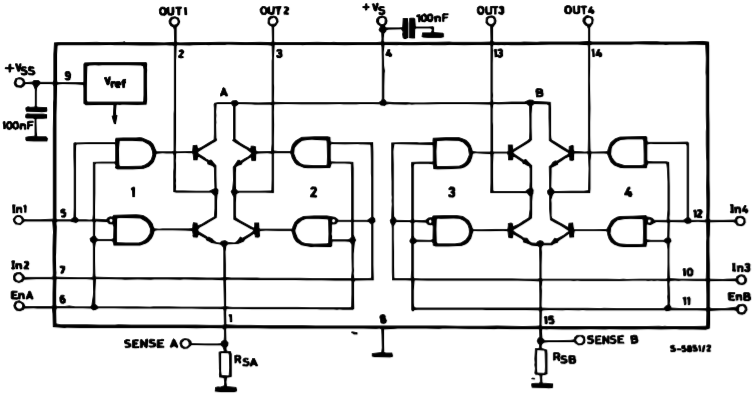
\includegraphics[scale=0.33]{tex/Design/L298}}
	\caption{L298 indeholdende to H-broer}
	\label{fig:L298}
\end{figure}

\noindent
Da boardsene aldrig kom til at fungere blev motor drivere af typen Pololu-A4988\footnote{Datablad for Pololu-A4988} taget i brug. Driveren følger samme princip som L298 med to H-broer, men motoren styres gennem et PWM-signal, en enable pin og en direction pin. Se databladet for Pololu-A4988 for yderligere information.

\subsection{Åbningsmekanisme}
\subsubsection{Hardware}
\myparagraph{Iskruning}
Ved at teste hvor stor en kraft der skal til for, at skrue proptrækkeren i proppen, kunne en aktuator vælges ud fra testen. Desværre for projektet har det været umuligt at finde ordentligt måleudstyr. Desuden har det ikke været muligt at sammenligne med lignende eksisterende produkter så et design af iskruning er aldrig opnået.

\myparagraph{Proptrækning}
Test af proptrækning med kraftmåler lånt fra Navitas giver et krav til motoren om moment på +25 kg.